\documentclass[11pt,a4paper]{article}
\usepackage[margin=2.2cm]{geometry}
\usepackage[T1]{fontenc}
\usepackage[utf8]{inputenc}
\usepackage{lmodern,microtype,amsmath,booktabs,tabularx,array,enumitem,xcolor,hyperref,fancyhdr,lastpage,graphicx,float}
\definecolor{accent}{HTML}{647687}\definecolor{navy}{HTML}{17365D}
\hypersetup{colorlinks=true,linkcolor=navy,urlcolor=navy,pdftitle={Zinc Certificate Valuation Research Report}}
\pagestyle{fancy}\fancyhf{}\lhead{Zinc Certificate Valuation}\rhead{Research Report}\cfoot{Page \thepage\ of \pageref{LastPage}}
\setlength{\headheight}{14pt}\setlist[itemize]{leftmargin=1.5em,itemsep=2pt}
\newcommand{\pct}{\,\%}\newcommand{\code}[1]{\texttt{#1}}
\graphicspath{{figures/}}
\begin{document}
\begin{titlepage}\centering
\vspace*{2cm}{\Huge\bfseries\color{accent} Zinc Certificate Valuation\par}
\vspace{0.5cm}{\LARGE Data, Methodology, Implementation, and Results\par}
\vspace{1cm}\rule{0.85\textwidth}{1pt}\par\vfill
{\large Iranian Mercantile Exchange zinc ingot certificate and physical market\par}
\vspace{0.3cm}{\large LME cash zinc and free-market USD/IRR\par}\vfill
\begin{tabular}{rl}\textbf{Data checkpoint:}&10 August 2026\\\textbf{Report date:}&10 August 2026\\\textbf{Status:}&Complete benchmark and three-bubble pipeline\end{tabular}
\vfill{\small Research documentation only; not investment advice.\par}
\end{titlepage}
\tableofcontents\newpage

\section{Executive Summary}
This project built a reproducible valuation pipeline for the Iranian zinc ingot warehouse
receipt. It integrates official IME certificate and physical-market data, LME cash zinc, and
free-market USD/IRR. The analytical underlying is a volume-weighted basket of 99.97 and 99.98
zinc ingots traded through cash and cash-matching contracts. Zinc soil and other grades remain
in broad raw data but are excluded from the ingot benchmark.

The principal result covers 178 modeled days from 26 October 2025 to 9 August 2026, with 41
exact anchors and 137 interpolated days. The certificate-to-estimated-physical bubble averaged
0.34\pct, had a median of 1.02\pct, ranged from $-19.58\pct$ to 16.97\pct, and was positive
on 102 days. By contrast, the certificate was below the simple LME--FX intrinsic proxy on all
182 certificate trading days, demonstrating why domestic physical basis must be modeled.

\section{Research Architecture and Data Governance}
Raw responses and canonical files are separated from derived outputs. Source snapshots are
immutable; collectors are incremental, idempotent, schema-validated, and atomic; zero offers
remain in raw; processed builders are deterministic; and notebooks are read-only presentation
layers. Shared IME logic is in \code{shared/ime\_data}, while zinc identity and grade rules remain
explicit in \code{commodity/zinc}.

\section{Data Sources and Collection Logic}
\subsection{Certificate}
The official IME CDC endpoint is \url{https://dataapi.ime.co.ir/api/CDC/CDCTrades}.
Codes \code{CD1ZNI0001} and \code{ZincIngot} form one continuous series with Commodity ID 30.
The collector refreshes 14 trailing days, preserves zero-volume days and complete JSON snapshots,
merges by date, validates schema/identity, and writes atomically. \code{TodaySettlementPrice} is
the analytical price; \code{TradesValue/TradesVolume} is only a rounding-tolerant validation.
The current file has 252 calendar rows through 9 August 2026 and 182 positive-trade days.

\subsection{Broad physical zinc raw data}
The official monthly IME physical endpoint is archived before filtering. Raw selection keeps
normalized goods names containing zinc, intentionally retaining both zinc ingot and zinc soil.
It does not impose grade, producer, symbol, settlement, or contract restrictions. The current
raw CSV has 6,235 rows, 3,462 positive trades, and 1,003 dates through 1405/05/18.

The latest healthy snapshot for each of 233 months can rebuild the exact CSV. A damaged older
snapshot for 1403/11 is preserved under the immutability policy; a later healthy snapshot for
the same month is selected during rebuild.

\subsection{LME and FX}
Westmetall is queried with \code{LME\_Zn\_cash}. Annual HTML snapshots are preserved, source
missing markers remain raw, and incremental refresh touches only the newest year. The current
LME file contains 4,704 unique dates from 2 January 2008 through 7 August 2026.

The canonical FX file stores IRR/USD. Recent TGJU observations use daily close; 13,030 historical
midpoint observations remain explicitly labeled legacy. The file contains 13,064 dates through
1405/05/17, including 34 close-based observations.

\section{Underlying Selection and Physical Benchmark}
Exploration showed that zinc soil dominates the broad zinc-labelled volume but is not the
warehouse receipt's underlying. Zinc ingots also span several grades, producers, and symbols.
The approved benchmark therefore includes:
\begin{itemize}
\item zinc ingot grades 99.97 and 99.98 only;
\item cash and cash-matching contracts only;
\item positive price and quantity;
\item all eligible producers/symbols, volume weighted within each day.
\end{itemize}
No single producer is selected without documentary equivalence. Daily price is
\begin{equation}P_d=\frac{\sum_i p_{i,d}q_{i,d}}{\sum_i q_{i,d}}.\end{equation}
The resulting \code{zinc\_9798\_cash\_daily.csv} has 554 days from 16 August 2009 to
9 August 2026: 239 with both grades, 158 with only 99.97, and 157 with only 99.98.
Eligible volume totals 155,602 tonnes: 71,852 tonnes of 99.97 and 83,750 tonnes of 99.98.

\section{Intrinsic Price and As-of Alignment}
The latest LME cash and FX observation on or before each target date is joined without future
information. Source date and age are retained. Maximum observed LME age is four days; maximum
FX age is ten days over the full benchmark and one day in the certificate period. Intrinsic value is
\begin{equation}I_t=\left(\frac{LME^{cash}_t}{1000}\right)FX_t\quad\text{IRR/kg}.\end{equation}
It is a transparent market factor, not a full domestic parity price.

\section{Three Bubble Definitions}
\begin{align}
B^{P/I}_t&=100\left(\frac{P_t}{I_t}-1\right),\\
B^{C/I}_t&=100\left(\frac{C_t}{I_t}-1\right),\\
B^{C/P}_t&=100\left(\frac{C_t}{\widehat{P}_t}-1\right).
\end{align}
These respectively measure domestic physical basis, direct certificate basis to LME--FX, and
the principal certificate premium to estimated domestic physical value.

\section{Primary Estimator: Ratio Interpolation}
For exact certificate/physical anchors, $R_a=P_a/I_a$. Between adjacent anchors:
\begin{align}
w_t&=\frac{t-a_L}{a_R-a_L},\\
\widehat{R}_t&=R_{a_L}+w_t(R_{a_R}-R_{a_L}),\\
\widehat{P}_t&=\widehat{R}_t I_t.
\end{align}
The method interpolates on calendar time, reconstructs observed anchors, and never extrapolates
outside the first/last anchor. LME and FX variation continues to enter through $I_t$.

\section{Experimental Regression}
The only feature is intrinsic price; target is physical benchmark price; certificate price is
not fitted. Five-fold time-series cross-validation compares proportional, intercept-linear, and
degree-two ridge models. The selected model is proportional without intercept, with RMSE
256,696.52 IRR/kg. Regression remains experimental because anchor history is limited; ratio
interpolation is official.

\section{Results}
\begin{table}[h]\centering
\begin{tabular}{lrrrrrr}\toprule
Measure&Rows&Mean&Median&Minimum&Maximum&Pos./Neg.\\\midrule
Physical vs intrinsic&554&$-13.14\pct$&$-15.87\pct$&$-36.02\pct$&22.28\pct&75/479\\
Certificate vs intrinsic&182&$-20.13\pct$&$-18.58\pct$&$-33.91\pct$&$-10.54\pct$&0/182\\
Certificate vs est. physical&178&0.34\pct&1.02\pct&$-19.58\pct$&16.97\pct&102/76\\
Regression sensitivity&182&0.58\pct&2.53\pct&$-16.77\pct$&12.66\pct&104/78\\\bottomrule
\end{tabular}\caption{Zinc bubble results}\end{table}

The persistent certificate discount to intrinsic largely mirrors a domestic physical discount.
Once that basis is incorporated, the mean principal certificate bubble is near zero, though its
range remains economically material.

\section{Visual Analysis of the Three Bubble Measures}

\subsection{Physical market versus intrinsic value}
Figure~\ref{fig:zn-physical} presents all 554 days in the approved 99.97/99.98 physical
benchmark. The physical basket trades below LME--FX intrinsic value on 479 days and above it
on 75. The persistent negative basis is an empirical characteristic of the domestic ingot
market and may reflect omitted costs, market segmentation, quality/delivery differences, and
the limitations of the parity proxy. It is not evidence that raw zinc soil belongs in the basket.

\begin{figure}[H]\centering
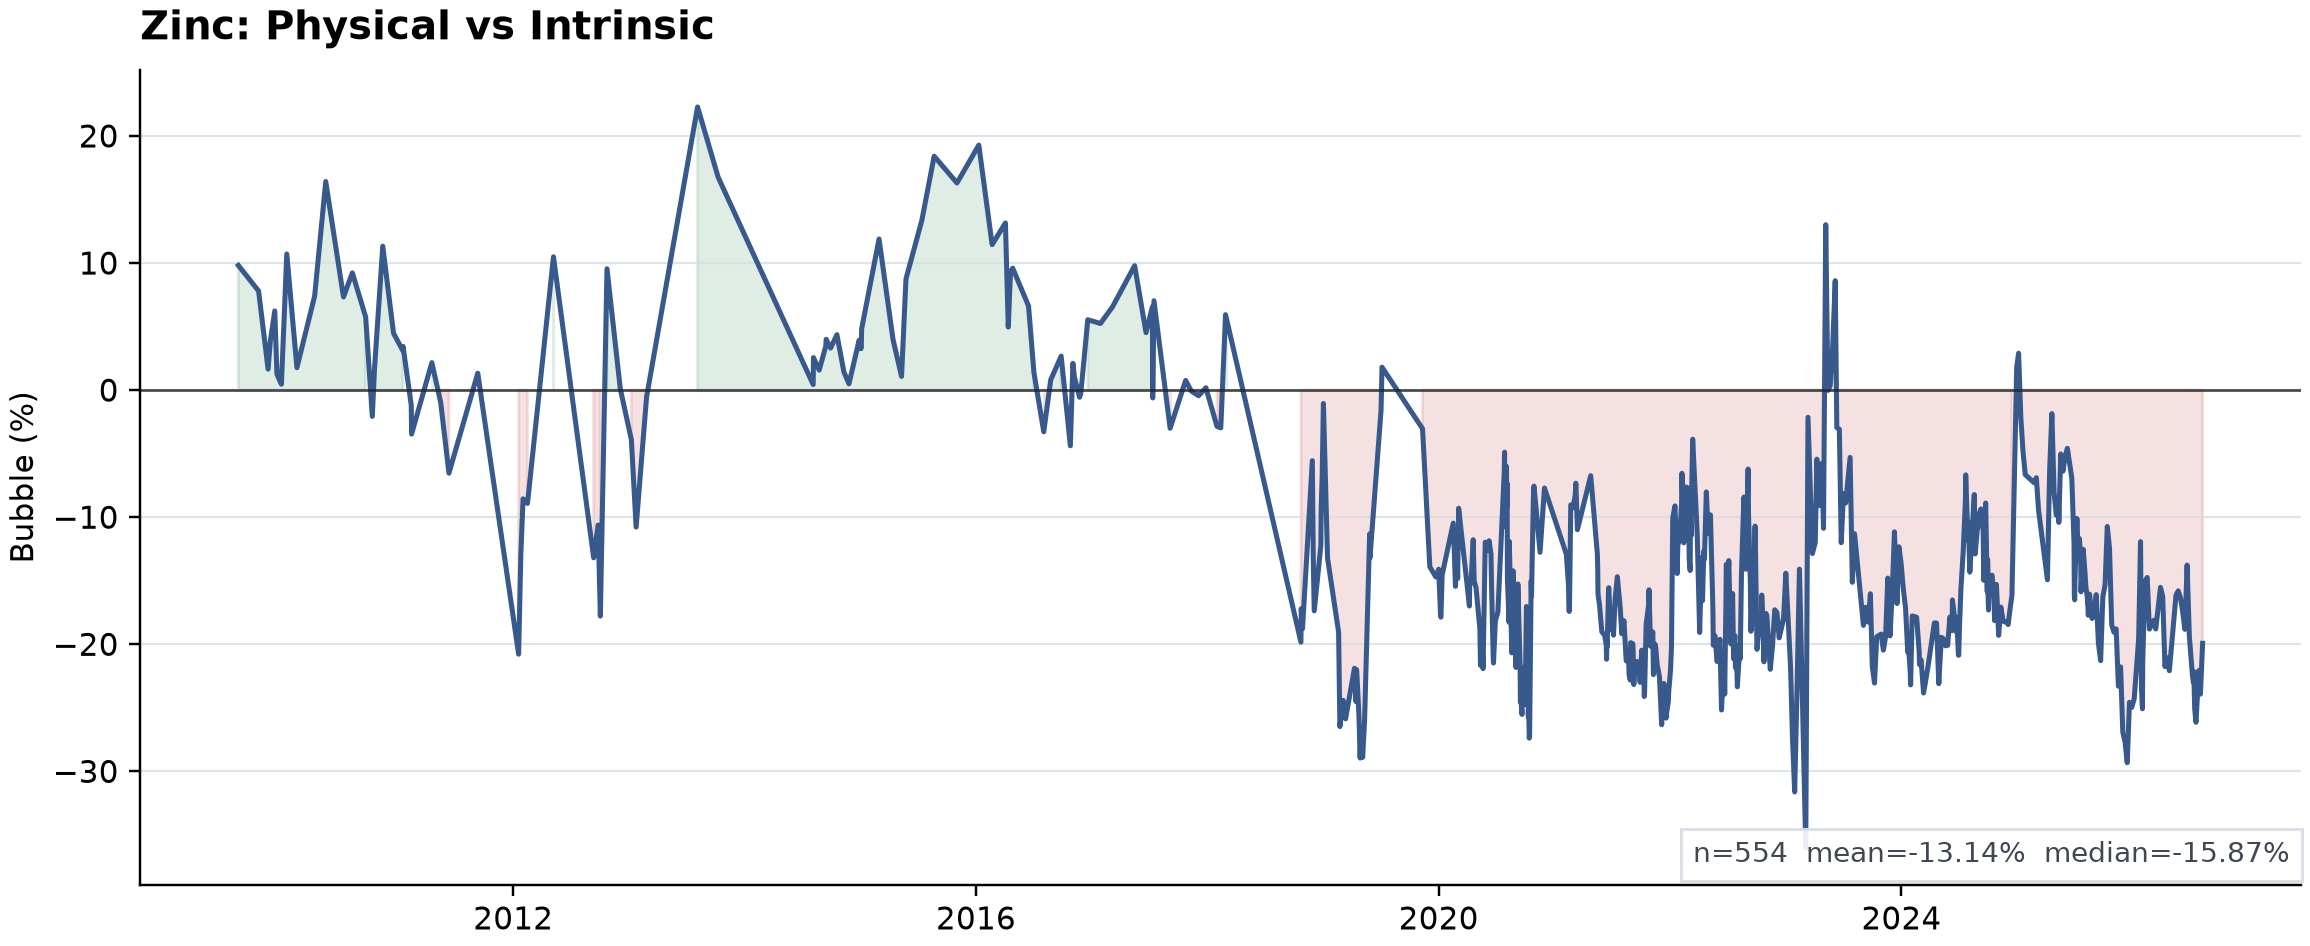
\includegraphics[width=0.97\textwidth]{zinc_physical_bubble.png}
\caption{Zinc 99.97/99.98 physical basket relative to LME--FX intrinsic value. The zero line
marks parity; green shading denotes a positive basis and red shading a discount.}
\label{fig:zn-physical}\end{figure}

\subsection{Certificate versus intrinsic value}
Figure~\ref{fig:zn-certificate} is negative for every one of the 182 positive-volume
certificate days. Its mean is $-20.13\pct$. Read alone, this chart might suggest a persistent
certificate discount. That conclusion is incomplete because the comparable domestic ingot
basket also trades at a material discount to the LME--FX proxy.

\begin{figure}[H]\centering
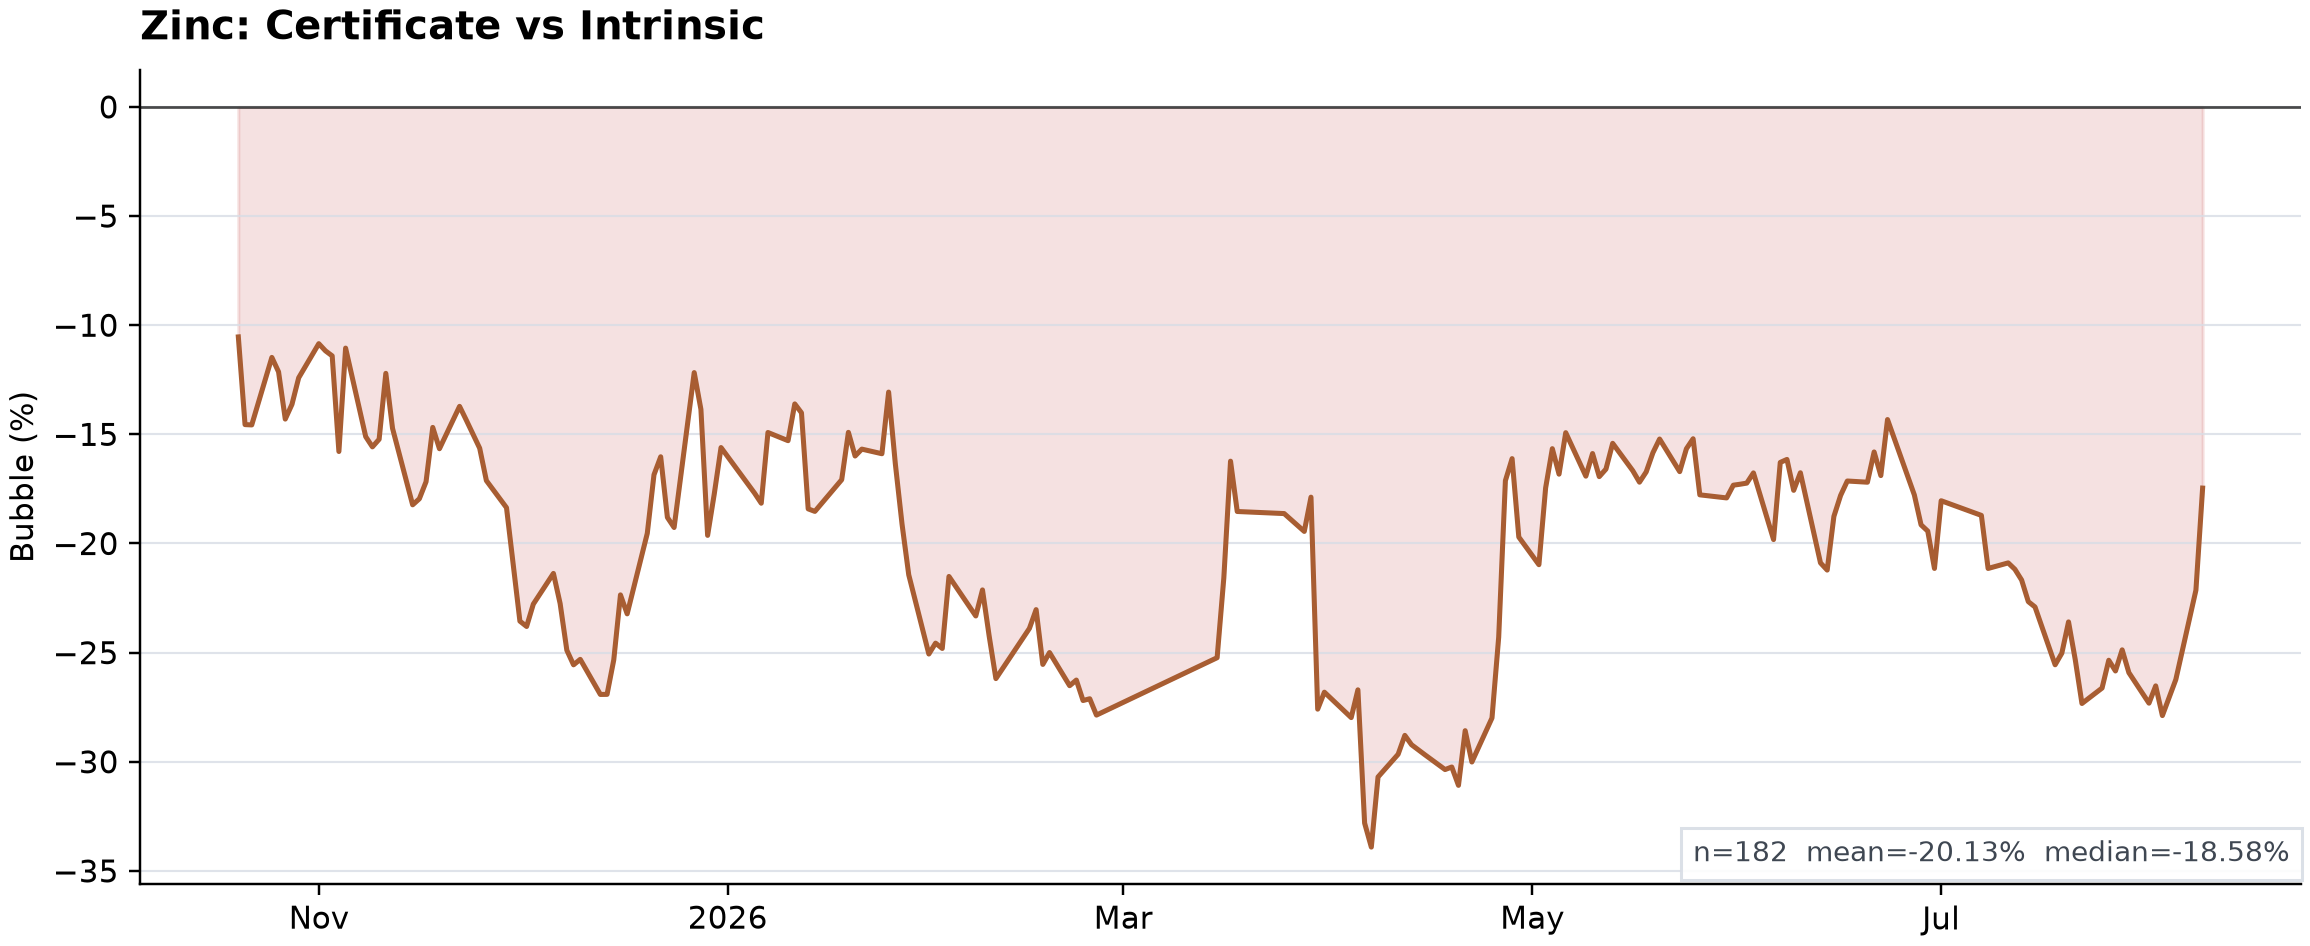
\includegraphics[width=0.97\textwidth]{zinc_certificate_bubble.png}
\caption{Zinc certificate settlement price relative to LME--FX intrinsic value.}
\label{fig:zn-certificate}\end{figure}

\subsection{Certificate versus estimated domestic physical value}
Figure~\ref{fig:zn-main} is the principal zinc valuation series. It uses 41 exact anchors and
137 calendar-time interpolations, with no extrapolation outside the observed anchor range. The
series oscillates around zero: 102 positive and 76 negative observations, a mean of 0.34\pct,
and a median of 1.02\pct. The near-zero center contrasts sharply with the uniformly negative
certificate/intrinsic chart and quantifies the importance of the domestic basis adjustment.

\begin{figure}[H]\centering
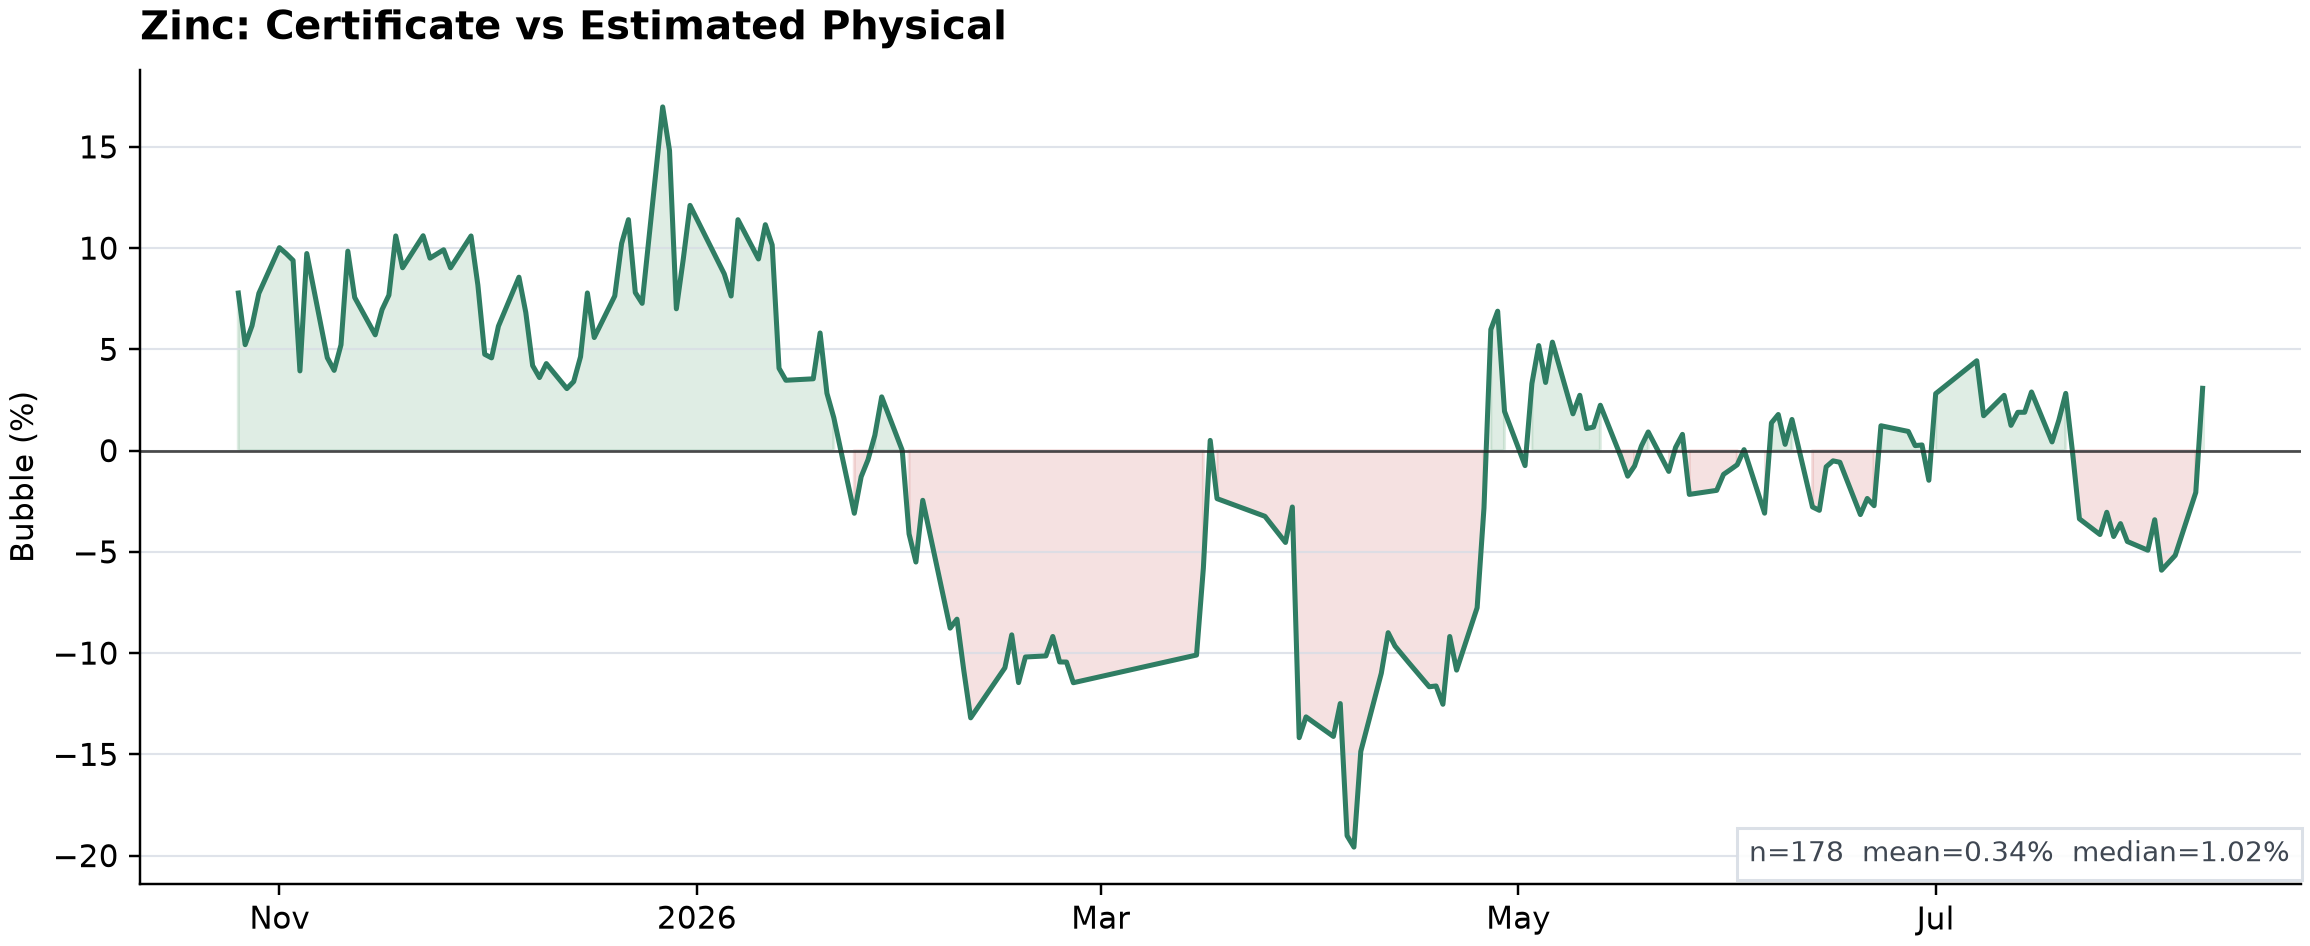
\includegraphics[width=0.97\textwidth]{zinc_main_bubble.png}
\caption{Principal zinc certificate bubble relative to the estimated 99.97/99.98 domestic
physical basket.}
\label{fig:zn-main}\end{figure}

\subsection{How to read the three charts together}
The first chart measures how the eligible domestic ingot basket differs from global zinc
translated at free-market FX. The second measures the certificate against that global factor.
The third compares certificate value with the estimated domestic basket after carrying the
physical basis through time. Consequently, a large negative direct intrinsic bubble can coexist
with a near-zero domestic-physical bubble. The physical line connects irregular trading dates;
the principal line includes interpolated basis ratios and must not be described as fully observed
physical prices.

\section{Validation, Tests, and Determinism}
Controls include schema and identity contracts, old/new code continuity, sorted unique dates,
calendar round trips, non-negative values, exact duplicate/business-key checks, settlement/VWAP
reconciliation, broad-raw versus narrow-benchmark separation, healthy latest-month snapshot
selection, as-of ages, anchor reconstruction, and no extrapolation. Fourteen network-free tests
cover raw contracts, LME, benchmark rules, three bubble formulas, anchors, regression, and rebuild
behavior. Repeated execution of all four processed builders produced identical hashes.

\section{Outputs and Reproduction}
The six analytical outputs are \code{zinc\_9798\_cash\_daily.csv},
\code{physical\_vs\_intrinsic\_bubble.csv},
\code{certificate\_vs\_intrinsic\_bubble.csv},
\code{zinc\_certificate\_bubble.csv}, \code{intrinsic\_regression.csv}, and
\code{intrinsic\_regression\_metrics.csv}. Run certificate, physical, LME, and FX collectors;
then build the benchmark, direct intrinsic bubbles, principal bubble, and regression in order.

\section{Limitations and Next Steps}
The 41-anchor sample is still limited. The 99.97/99.98 basket may retain producer, warehouse,
delivery, and quality effects. Ratio interpolation assumes a smooth domestic basis. Intrinsic
value excludes taxes, logistics, financing, storage, and liquidity. A modeled premium or discount
does not guarantee convergence.

Next steps are scheduled monitored refreshes, explicit LME/FX age thresholds, executed notebook
interpretation, monitoring grade/producer composition and anchor gaps, and revisiting eligibility
only when certificate specification and delivery documentation justify a change.

\section*{Provenance Note}
All figures were calculated from local canonical and processed CSVs at the stated checkpoint.
Raw snapshots remain immutable and unversioned by policy. No credentials are stored in this
document or project source.
\end{document}
